\section{Memory-augmented Online VAD\mnote{VAD viene risolto solo in fig. 1}}
\label{sec:theory}

\fboxsep=1mm%padding thickness
\fboxrule=1pt%border thickness

\begin{figure}[!t]
            \centerline{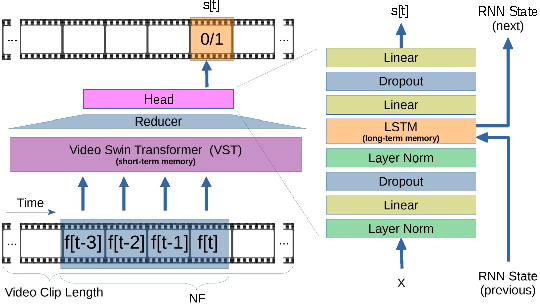
\includegraphics[clip, width=\linewidth]{images/arch-rx-cropped.pdf}}
        \caption{The online frame-level Video Anomaly Detection (VAD) architecture. $f[t]$ is the frame at time $t$, $x$ the output of the Reducer, $\mathit{NF}$ the number of frames in input to the VST, $s[t]$ the anomaly classification score of the frame $f[t]$.\label{fig:arch}}
\end{figure}

In this section the MOVAD architecture is described.  
The model is composed by: a short-term memory module and a classification head that includes a long-term  memory module (see Fig.~\ref{fig:arch}). 
Taking inspiration from~\cite{xu2021long}, recently observed frames have been taken into account as a source of information related to the ongoing action, and past frames as a source of information on the context.

\noindent\textbf{Short-term memory module.}
Since we are dealing with the online VAD task, the only information available to the system, at any given time, are the current and the past frames.
Only a small portion of these frames are used as input at each step.
In order to implement this module, we selected the Video Swin Transformer (VST)~\cite{liu_video_2022} over ViViT~\cite{Arnab_2021_ICCV} due to its superior performance, and over an RNN given its ability to process frames in parallel.
Originally borns to carry out the Video Action Classification task, analyzing all the frames in one step, we adapted to perform single frame classification using few of them.
In particular, it considers only a small temporal window of $\mathit{NF}$ frames of the video, going from the current frame at time $t$ to the previous frames at time $t-\left(\mathit{NF}-1\right)$.
As shown in Fig.~\ref{fig:arch}, in our case $\mathit{NF}=4$, i.e., the input of the VST is formed by $f[t]$, $f[t-1]$, $f[t-2]$ and $f[t-3]$, where $f[t]$ represents the frame at time $t$.
VST takes as input a video with size $\mathit{NF} \times H \times W \times 3$, where $\mathit{NF}$, $H$ e $W$ correspond to the number of frames, height, width and RGB channels, respectively.
The model internally splits the frames in non-overlapping 3D patches, partitioning the video in $\frac{\mathit{NF}}{2} \times \frac{H}{4} \times \frac{W}{4}$ 3D tokens, projecting the features to an arbitrary dimension $C$.
The rest of the architecture is similar to the original Swin Transformer~\cite{liu2021Swin}, with four stages of Video Swin Transformer blocks, interspersed with $2\times$ spatial down-sampling in the patch merging layer.

\noindent\textbf{Classification Head.}
The classification head generates the final output and  attached to the output of the VST after an Adaptive Average Pool 3D layer (Reducer in Fig.~\ref{fig:arch}).
As shown in Fig.~\ref{fig:arch}, the head is composed by a series of normalization layers, linear layers and dropout, alternating. 
The classification head also deals with long-term memory thanks to a LSTM module inserted after the last normalization layer.
For each frame $f[t]$, the model outputs the anomaly classification score $s_t \in [0,1]$, where $s_t=0$ means no anomaly and $s_t=1$ means the frame is surely anomalous.
A weighted cross-entropy loss was chosen, giving higher weight to the anomaly class, in order to reflect the distribution of the data.

In order to not lose information from the distant past, we need a way to keep track of it.
For this reason, we introduce a long-term memory module  which is updated whenever a new frame is analyzed by the system.
Specifically, we choose to employ a RNN module (LSTM \cite{lstm} in this specific case).
Given that the input of the LSTM  are only the latent features in output of the Reducer, the module is very efficient and leads to a limited additional computational cost.
Indeed, it condenses all its knowledge into two states: an hidden state $h_t$ and cell state $c_t$.
Since the output of the first linear layer of the classifier head provides the summary about the $\mathit{NF}$ frames processed by the short-term memory model, the LSTM cells is added after it.

% copyright image frame: <a href="https://www.freepik.com/free-vector/realistic-vector-icon-film-tape-strip-with-white-square-isolated-white-cinema-concept_31096470.htm#query=video%20frame&position=31&from_view=keyword">Image by user15245033</a> on Freepik